\section{Conclusion and Discussion}

\begin{frame}
  \tableofcontents[currentsection] 
\end{frame}


\begin{frame}[fragile]
 \heading{Conclusion}

\vspace{2ex}

odeint is a modern C++ library for solving ODEs that is
%odeint is a modern C++ library for solving ordinary differential equations, which is

\begin{itemize}
 \item easy-to-use
 \item highly-flexible
 \begin{itemize}
  \item data types (topology of the ODE, complex numbers, precision, \dots)
  \item computations (CPU, CUDA, OpenMP, ...)
 \end{itemize}
 \item fast
\end{itemize}





\end{frame}



\begin{frame}
 \heading{Where can \odeint\ be used?}

 \vspace{2ex}

 \begin{itemize}
  \item Science
  \item Game engine and physics engines
  \item Simulations
  \item Modelling
  \item Data analysis
  \item High performance computing
 \end{itemize}

\end{frame}


\rem{
\begin{frame}[fragile]
 
 \heading{Who uses odeint}

\vspace{4ex}



\begin{minipage}{0.2\textwidth}
 \begin{center}
  NetEvo

  \vspace{1ex}
  
  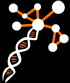
\includegraphics[draft=false,width=1.0\textwidth]{netevo.png}
 \end{center}
\end{minipage}
\hspace{2ex}\begin{minipage}{0.3\textwidth}
 \begin{center}
  \textbf{OMPL} -- Open Motion Planning Library
 \end{center}
\end{minipage}
\hspace{2ex}\begin{minipage}{0.3\textwidth}
 \begin{center}
   \textbf{icicle} -- cloud/precipitation model
 \end{center}
\end{minipage}


\end{frame}
}

\begin{frame}[fragile]
 
 \heading{Who uses odeint}

\vspace{2ex}


\textbf{NetEvo} -- Simulation dynamical networks

\vspace{2ex}
\textbf{OMPL} -- Open Motion Planning Library

\vspace{2ex}
\textbf{icicle} -- cloud/precipitation model

\vspace{2ex}
\textbf{Score} -- Commercial Smooth Particle Hydrodynamics Simulation

\vspace{2ex}
\textbf{VLE} -- Virtual Environment Laboratory (planned to use \odeint )

\vspace{2ex}
Several research groups

\vspace{2ex}
\dots


\end{frame}





\begin{frame}
 \heading{Roadmap}

 \vspace{2ex}

Near future:
\begin{itemize}
\item Current release -- documentation, bug fixing
\item Boost Review process
\item Implicit steppers
\end{itemize}

\vspace{2ex}
Further plans 
\begin{itemize}
 \item Dormand-Prince 853 steppers
 \item More algebras: MPI, cublas, TBB, John Maddock's arbitrary precision library, Boost SIMD library
\end{itemize}

\vspace{2ex}                                                                                                       
Persepective
\begin{itemize}
 \item C++11 version
 \item sdeint -- methods for stochastic differential equations
 \item ddeint -- methods for delay differential equations
\end{itemize}







\end{frame}
